\chapter{Podwarstwa Packet Data Convergence Protocol}
\label{cha:pdcp}

Podwarstwa PDCP (Packet Data Convergence Protocol) jest pierwszą z podwarstw z których składa się warstwa 2 stosu protokołów LTE. Dla każdego nośnika radiowego konfigurowana jest jej osobna instancja. Może ona odpowiadać za dane na płaszczyźnie użytkownika (wówczas świadczy usługi dla warstwy IP) lub za dane na płaszczyźnie kontroli i wówczas korzysta z niej warstwa RRC. Warstwa PDCP używa warstwy RLC do dalszej komunikacji.

W zależności od płaszczyzny danych, warstwa PDCP jest odpowiedzialna za:

Dla płaszczyzny kontroli:
\begin{enumerate}
	\item Dostarczenie danych w odpowiedniej kolejności i bez duplikatów
	\item Zapewnienie integralności danych
	\item Szyfrowanie danych
\end{enumerate}

Dla płaszczyzny danych użytkownika:
\begin{enumerate}
	\item Dostarczenie danych w odpowiedniej kolejności i bez duplikatów
	\item Kompresję nagłówków
	\item Szyfrowanie danych
\end{enumerate}

W projekcie skupiono się na symulacji przesyłu danych na płaszczyźnie danych użytkownika. Poniżej opisano proces przesyłu pakietu IP od urządzenia użytkownika (UE) do stacji bazowej (eNB) z perspektywy podwarstwy PDCP. Pomocniczo posłużono się zrzutami ekranu z wykonanej symulacji.

\section{Przetwarzanie pakietów IP na podwarstwie PDCP}

Pierwszym krokiem po otrzymaniu pakietu z warstwy IP w obrębie podwarstwy PDCP jest nadanie otrzymanej jednostce danych numeru. Przypisany numer pozwala podwarstwie PDCP po stronie odbiornika odrzucić zduplikowane jednostki danych oraz dostarczyć je do wyższych warstw w odpowiedniej kolejności.

\begin{figure}
	\centering
		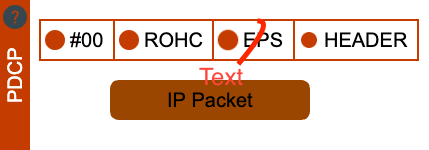
\includegraphics[width=0.5\textwidth]{pdcp.png}
	\caption{PDCP}
\end{figure}

Drugim krokiem jest kompresja nagłówka pakietu IP przy użyciu metody ROHC (Robust Header Compression). Ogólna zasada działania opiera się na założeniu, że jeżeli pakiety IP wysyłane są pomiędzy dwoma urządzeniami wówczas większość pól w ich nagłówkach jest taka sama. W przypadku pakietu IPv4 rozmiar nagłówka wynosi 20 bajtów. Jeżeli jest on użyty w połączeniu z protokołami UDP i RTP wówczas rozmiar nagłówka w sumie wynosi 40 bajtów. ROHC pozwala zmniejszyć rozmiar takiego nagłówka do 2 - 4 bajtów. Warto również zauważyć, że protokół RTP używany zazwyczaj w kodowaniu głosu w czasie rzeczywistym transportuje niewielkie ilości danych - zazwyczaj 20 - 40 bajtów. Porównując to z nieskompresowanym nagłówkiem o ilości 40 bajtów widać, że narzut nagłówka jest znaczny. Dzięki temu zastosowanie kompresji ROHC pozwala zaoszczędzić znaczną część pasma.

Po kompresji następuje szyfrowanie danych zawartych w pakiecie

Ostatnim krokiem jest dodanie nagłówka 